% --- Slide 1: FOMM Overview ---
\begin{frame}{First Order Motion Model (Siarohin et al., NeurIPS 2019)}
    \begin{columns}[c]
        \begin{column}{0.54\textwidth}
            \textbf{Core Innovations}
            \begin{itemize}
                \item \textbf{No Pretrained Landmarks:} Doesn't need 68 facial landmark detectors or 3D face models (3DMM).
                \item \textbf{Self-Supervised:} Learns keypoints automatically from raw video pairs.
                \item \textbf{Appearance / Motion Decoupling:} Appearance comes from source $S$; motion comes from driving $D$.
                \item \textbf{Generalizes Across Domains:} Works on human faces, bodies (Tai-Chi), and animals.
            \end{itemize}
        \end{column}

        \begin{column}{0.44\textwidth}
            \centering
            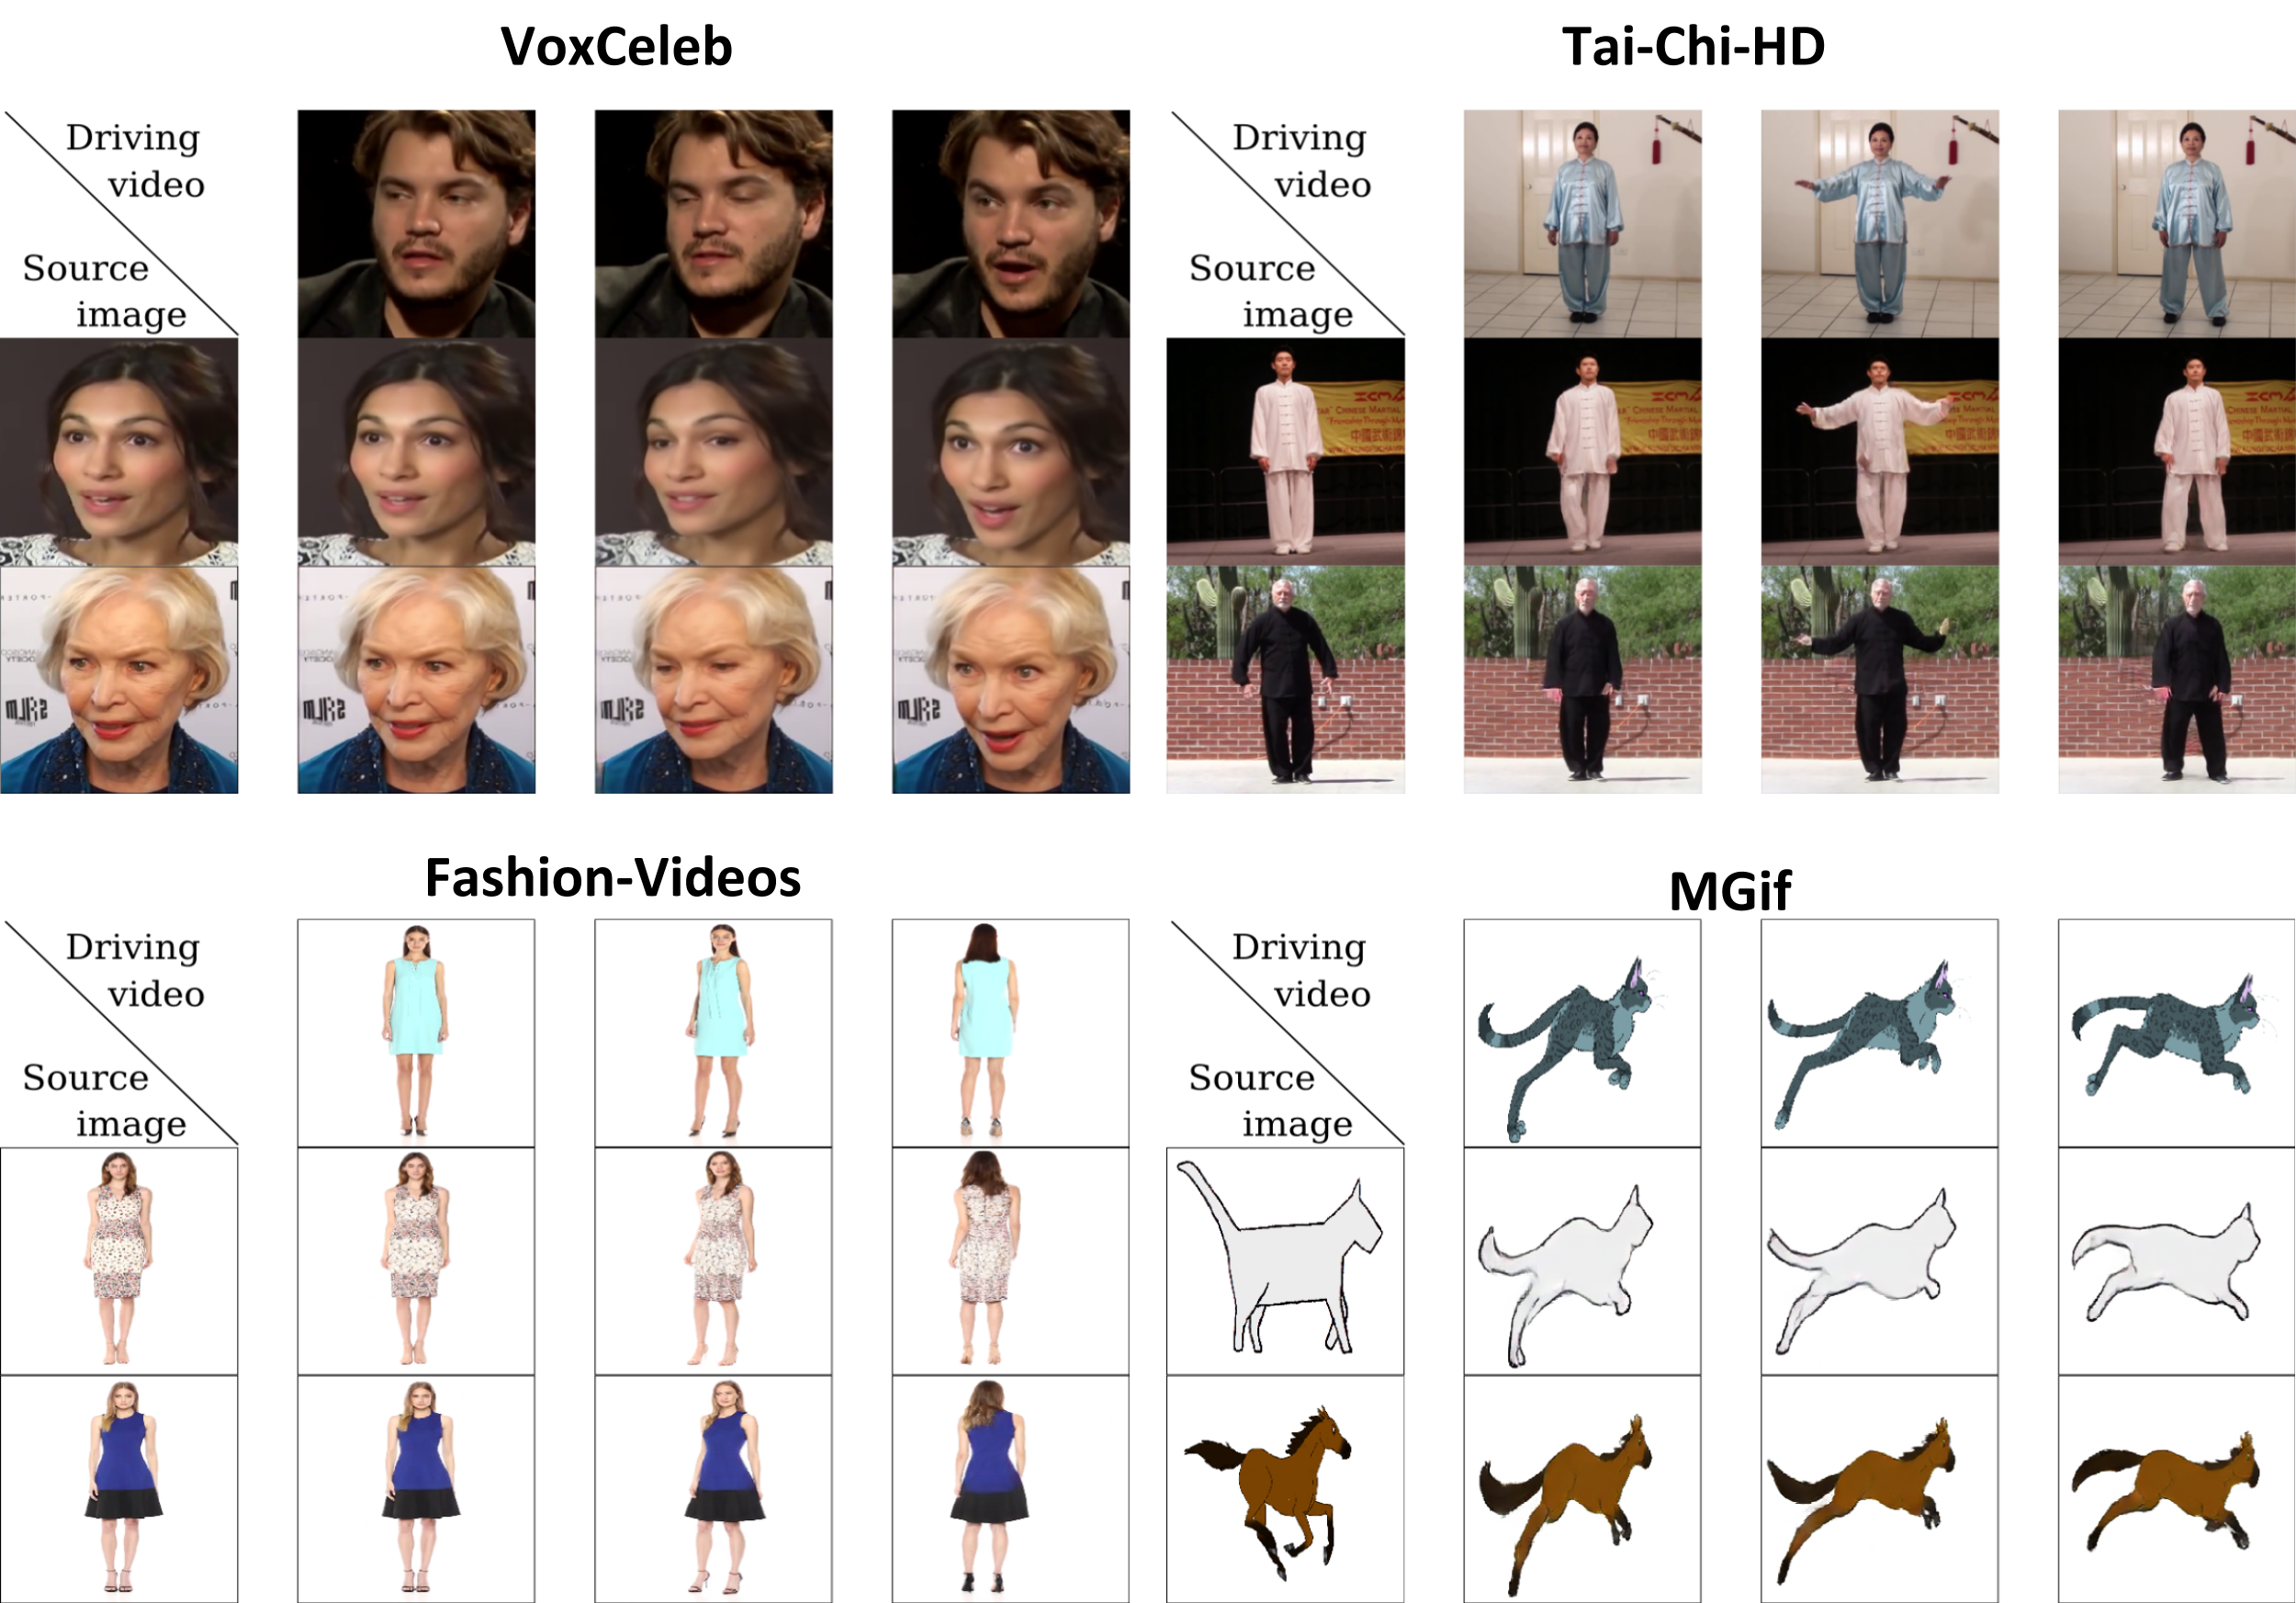
\includegraphics[width=\linewidth, height=3.8cm, keepaspectratio]{fomm_teaser.png}
            \vspace{0.15cm}
            
            \scriptsize \textit{FOMM teaser: VoxCeleb, Tai-Chi, Fashion (Siarohin et al., 2019).}
        \end{column}
    \end{columns}
\end{frame}

% --- Slide 2: Motion Representation: 0th vs 1st Order ---
\begin{frame}{Motion Representation: 0th-Order vs. 1st-Order Motion}
    \begin{columns}[c]
        \begin{column}{0.48\textwidth}
            \textbf{Motion Representation}
            \begin{itemize}
                \item \textbf{0th-Order (Translation Only):}
                \begin{itemize}
                    \item Moves points in 2D space $(x, y)$.
                    \item Cannot stretch skin; movement looks stiff and robotic.
                \end{itemize}
                \vspace{0.25cm}
                \item \textbf{1st-Order (FOMM):}
                \begin{itemize}
                    \item Tracks deformation around each point.
                    \item Captures rotation (head tilts), scale (mouth opening), and shear (skin stretch).
                \end{itemize}
            \end{itemize}
        \end{column}

        \begin{column}{0.50\textwidth}
            \centering
            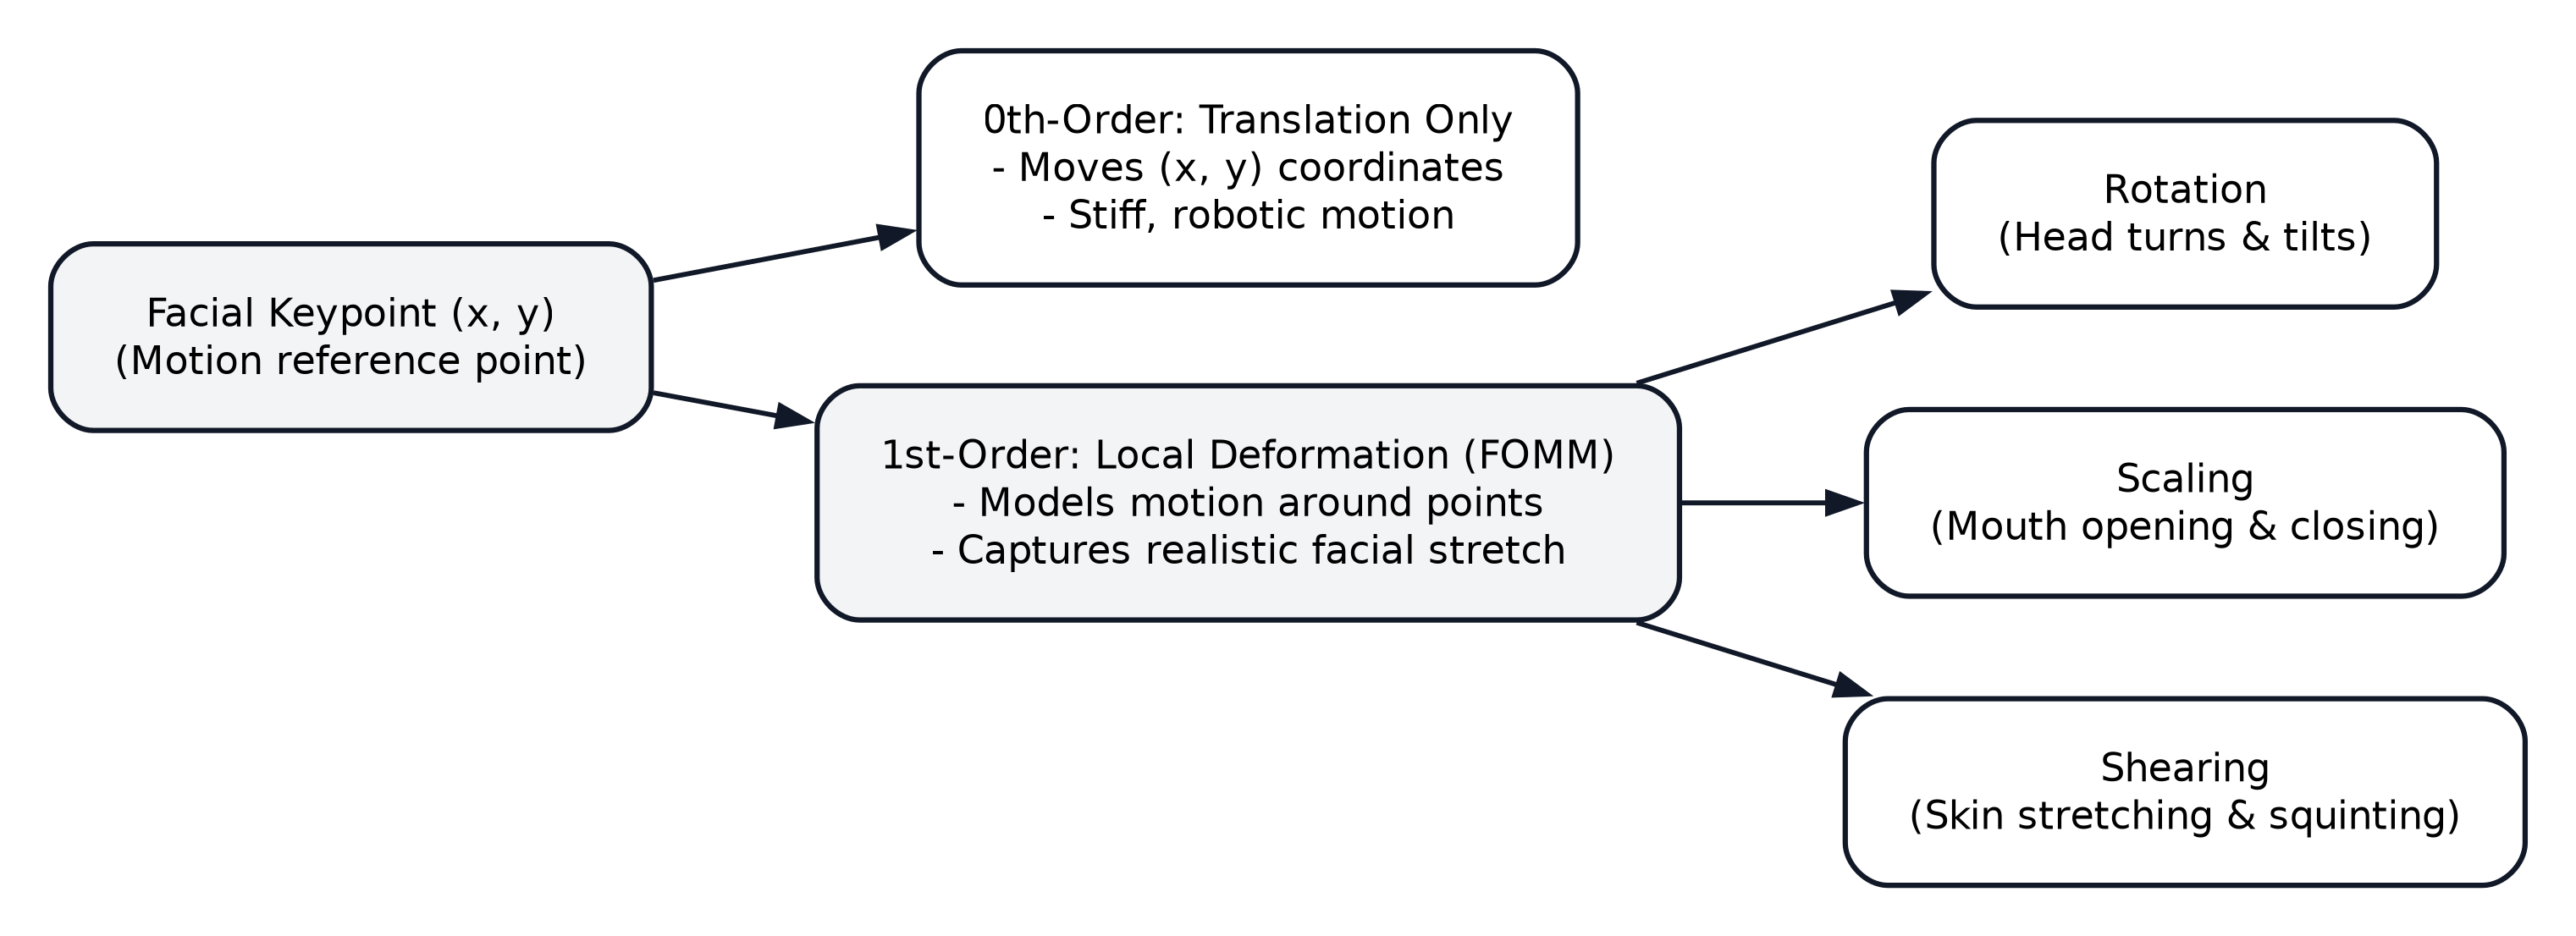
\includegraphics[width=\linewidth, height=4.2cm, keepaspectratio]{diagram_facial_motion_order.png}
        \end{column}
    \end{columns}
\end{frame}

% --- Slide 3: The FOMM Pipeline & Core Components ---
\begin{frame}{FOMM Architectural Pipeline}
    \begin{center}
        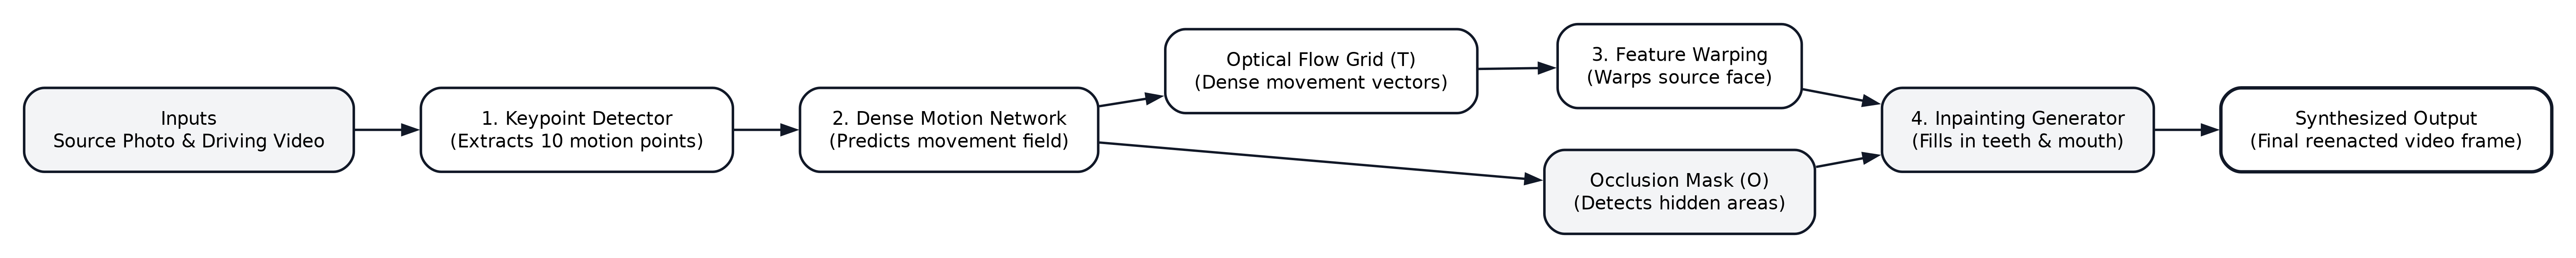
\includegraphics[width=0.96\linewidth, height=3.0cm, keepaspectratio]{diagram_fomm_pipeline.png}
    \end{center}

    \vspace{0.15cm}

    \begin{columns}[T]
        \begin{column}{0.32\textwidth}
            \begin{block}{1. Keypoint Detector}
                \scriptsize Hourglass network detects $K=10$ unsupervised keypoints and Jacobians.
            \end{block}
        \end{column}
        \begin{column}{0.32\textwidth}
            \begin{block}{2. Dense Motion Network}
                \scriptsize Converts sparse points into optical flow ($T$) and an occlusion mask ($O$).
            \end{block}
        \end{column}
        \begin{column}{0.32\textwidth}
            \begin{block}{3. Inpainting Generator}
                \scriptsize Warps source features using $T$ and inpaints occluded areas ($O \approx 0$).
            \end{block}
        \end{column}
    \end{columns}
\end{frame}
